\makeatletter\def\input@path{
	{./Graphics/}
}\makeatother%%
%
\documentclass[12pt,a4paper]{report} 
\usepackage{graphicx,amsmath,physics,fancyhdr,booktabs,hyperref}
\usepackage[T1]{fontenc}
\usepackage[utf8]{inputenc}
\usepackage[french]{babel}
\usepackage[svgnames,x11names,rgb,table]{xcolor}
\usepackage[margin=2cm,includefoot,includehead]{geometry}
\usepackage[hybrid,texMathDollars,texMathSingleBackslash,rawAttribute]{markdown}
\usepackage{tikz,tikzscale}
\usetikzlibrary{shapes.geometric, arrows, positioning, shadows, fit}
%
\hypersetup{ 
	colorlinks=true, 	% colorise les liens 
	breaklinks=true,	% permet le retour la ligne dans les liens trop longs 
	urlcolor= Blue3,  	% couleur des hyperliens (inclut dans x11names de xcolor
	linkcolor= Blue3, 	% couleur des liens internes 
	citecolor=Blue3,	% couleur des liens de citation
	%   bookmarksopen=true,	% ouvre les signets PDF au départ 
	pdfauthor={Nana Engo},	% Nom de l'auteur du texte
	pdfsubject={Chimie quantique computationnelle},%
	pdfkeywords={Hamiltonien, Approximation BO, HF, Etat fondamental, Etat excité}, % Mots clés
	pdftitle=Fondements et méthodes en chimie quantique computationnelle V2411 % Titre
}
% Prise en compte du numéro de la section dans les différentes numérotations
\numberwithin{equation}{section}
\numberwithin{figure}{section}
\numberwithin{table}{section}
%
\frenchbsetup{StandardLayout}
%
\setcounter{secnumdepth}{3} % Pour inclure les sous-sections
\renewcommand{\thesection}{\arabic{section}} % Numérotation des sections

%
\title{\textcolor{blue}{Fondements et méthodes en chimie quantique computationnelle}}
\author{Nana Engo\\serge.nana-engo@facsciences-uy1.cm\\
Département de Physique\\ Université de Yaoundé I}
%
\date{
    \vspace{8cm} % Espace avant les logos
    \begin{center}
        \begin{minipage}{0.3\textwidth}
        \centering
            
\includegraphics[width=.5\textwidth]{Neo_Logo.jpg}
        \end{minipage}
        \hfill
        \begin{minipage}{0.3\textwidth}
        \centering
        Novembre 2024
        \end{minipage}
        \hfill % Séparation entre les logos
        \begin{minipage}{0.3\textwidth}
        \centering
            
\includegraphics[width=.4\textwidth]{UY1_Logo}
        \end{minipage}
    \end{center}
}

%\titlegraphic{\includegraphics{Neo_logo.jpg}}

\begin{document}
\fancypagestyle{logo}{
\fancyhf{}
\fancyhead[LE,LO]{\includegraphics[scale=.3]{Neo_logo}}
\fancyhead[RE,RO]{\thepage}
\fancyhead[C]{Nana Engo}
}
\pagestyle{logo}

\arrayrulecolor{LawnGreen}\renewcommand{\arraystretch}{1.2}

\maketitle\begin{markdown}


## Fondements de la chimie quantique

En chimie quantique, l'équation fondamentale est celle de Schrödinger dépendant du temps :
\begin{equation}
i\hbar \pdv{t} |\psi(t)\rangle = \hat{H} |\psi(t)\rangle .
\end{equation}
Cette équation décrit comment la fonction d'état $|\psi(t)\rangle$ évolue dans le temps sous l'action de l'Hamiltonien $\hat{H}$. Cependant, résoudre cette équation dans sa forme générale est complexe, même en négligeant les effets relativistes.

Pour simplifier, on se concentre souvent sur l'équation de Schrödinger indépendante du temps, un problème aux valeurs propres :
\begin{equation}
\hat{H} |\psi\rangle = E |\psi\rangle .
\end{equation}
Ici, l’Hamiltonien $\hat{H}$ est exprimé comme suit, en unités atomiques (où la charge de l'électron, la masse de l'électron et $\hbar$ sont égales à 1) (voir la \autoref{fig:interactionqc}):
```{=tex}
\begin{equation}
\hat{H} = -\sum_{i=1}^N \frac12 \nabla_i^2 - \sum_{A=1}^M \frac{1}{2M_A} \nabla_A^2 - \sum_{i=1}^N \sum_{A=1}^M \frac{Z_A}{r_{iA}} + \sum_{i=1}^N \sum_{j>i} \frac{1}{r_{ij}} + \sum_{A=1}^M \sum_{B>A} \frac{Z_A Z_B}{R_{AB}} .
\end{equation}
```
où,
- $N$ est le nombre d'électrons;
- $M$ est le nombre de noyaux;
- $M_A$ est le rapport entre la masse du noyau $A$ et celle de l'électron;
- $Z_A$ est le numéro atomique du noyau $A$;
- $r_{iA}$ est la distance entre l’électron $i$ et le noyau $A$;
- $R_{AB}$ est la distance entre les noyaux $A$ et $B$.

\begin{figure}[tbph]
\centering
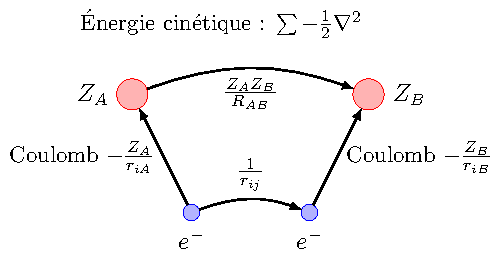
\includegraphics[width=0.7\linewidth]{Interaction_QC.pdf}
\caption{Illustration simplifiée des différentes interactions (électron-noyau, électron-électron, noyau-noyau) dans un système moléculaire.}
\label{fig:interactionqc}
\end{figure}

Les différents termes de l'Hamiltonien sont,
1. **Énergie cinétique des électrons**
   \begin{equation}
   -\sum_{i=1}^N \frac12 \nabla_i^2.
   \end{equation}

2. **Énergie cinétique des noyaux**
   \begin{equation}
   -\sum_{A=1}^M \frac{1}{2M_A} \nabla_A^2 .
   \end{equation}

3. **Interaction Coulombienne électron-noyau**
   \begin{equation}
   -\sum_{i=1}^N \sum_{A=1}^M \frac{Z_A}{r_{iA}} .
   \end{equation}

4. **Répulsion électron-électron**
   \begin{equation}
   \sum_{i=1}^N \sum_{j>i} \frac{1}{r_{ij}} .
   \end{equation}

5. **Répulsion noyau-noyau**
   \begin{equation}
   \sum_{A=1}^M \sum_{B>A} \frac{Z_A Z_B}{R_{AB}} .
   \end{equation}

L'équation de Schrödinger dans sa forme complète est inapplicable directement pour des systèmes multi-électrons. Des approximations sont nécessaires pour rendre les calculs réalisables.


## Approximation de Born-Oppenheimer

L'**approximation de Born-Oppenheimer** est une hypothèse fondamentale en chimie quantique, qui simplifie le traitement des systèmes moléculaires complexes. Elle repose sur la grande différence de masse entre les noyaux et les électrons. Les noyaux, étant bien plus massifs que les électrons, se déplacent beaucoup plus lentement. Cette différence de dynamique permet de séparer les mouvements électroniques et nucléaires dans l’équation de Schrödinger (voir la \autoref{fig:bointeractionqc}.

\begin{figure}[tbph]
\centering
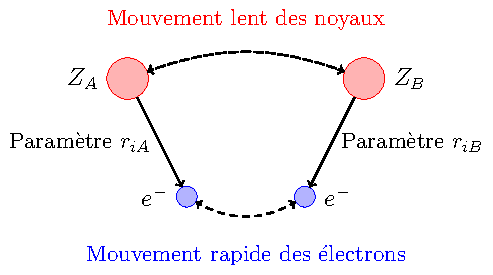
\includegraphics[width=0.7\linewidth]{BO_Interaction_QC.pdf}
\caption{Illustration des interactions dams l'approximation de Born-Oppenheimer.}
\label{fig:bointeractionqc}
\end{figure}

### Hamiltonien réduit

En appliquant cette approximation, le Hamiltonien électronique est extrait de l'Hamiltonien total :
```{=tex}
\begin{equation}
\hat{H}_{\text{elec}} = -\sum_{i=1}^N \frac12 \nabla_i^2 - \sum_{i=1}^N \sum_{A=1}^M \frac{Z_A}{r_{iA}} + \sum_{i=1}^N \sum_{j>i} \frac{1}{r_{ij}} .
\end{equation}
```
Cet Hamiltonien électronique dépend explicitement des positions des électrons, mais les positions des noyaux y apparaissent uniquement comme des paramètres fixes. Ainsi, l'énergie électronique $(E_{\text{elec}})$ est calculée pour une configuration donnée des noyaux.

### Énergie totale du système

Une fois l'énergie électronique obtenue, l'énergie totale est exprimée comme suit :
```{=tex}
\begin{equation}
E_{\text{tot}} = E_{\text{elec}} + \sum_{A=1}^M \sum_{B>A} \frac{Z_A Z_B}{R_{AB}},
\end{equation}
```
où,
- $E_{\text{elec}}$ est l'énergie électronique (résultat du Hamiltonien électronique);
- le second terme représente l'énergie de répulsion entre les noyaux, considérés comme des charges ponctuelles fixes.

### Conséquences de l'approximation

- L'énergie totale est calculée pour une géométrie nucléaire fixe.
- Les mouvements des noyaux (vibration, rotation, translation) peuvent être traités séparément en utilisant un Hamiltonien nucléaire effectif :
```{=tex}
\begin{equation}
\hat{H}_{\text{nucl}} = -\sum_{A=1}^M \frac{1}{2M_A} \nabla_A^2 + E_{\text{tot}}(\{R_A\}) .
\end{equation}
```
Ici, $E_{\text{tot}}(\{R_A\})$ agit comme un potentiel pour le mouvement des noyaux.

En résumé, l'approximation de Born-Oppenheimer est essentielle pour séparer les degrés de liberté nucléaires et électroniques, rendant ainsi le problème beaucoup plus gérable en chimie quantique computationnelle.


## Types d'excitations

En chimie quantique, l'étude des états excités implique de comprendre les différentes façons dont un électron peut être excité dans une molécule. Les excitations électroniques se produisent lorsque des électrons sont transférés d'un orbital occupé vers un orbital inoccupé, et elles influencent directement les propriétés optiques et spectroscopiques des systèmes étudiés.

\begin{figure}[htpb]
\centering
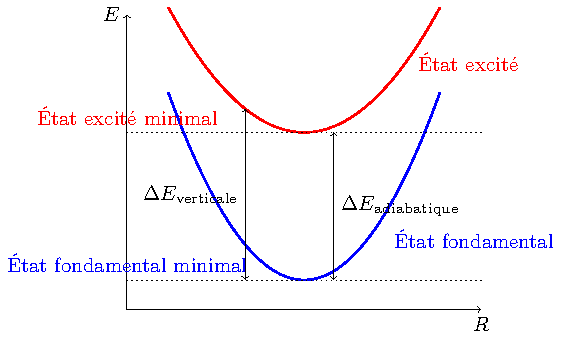
\includegraphics[width=0.7\linewidth]{Excited_states.pdf}
\caption{Illustration des différences entre $\Delta E_{\text{vertical}}$ et $\Delta E_{\text{adiabatic}}$.}
\label{fig:excitedstates}
\end{figure}

Deux types principaux d'énergies d'excitation sont distingués (voir la \autoref{fig:excitedstates}):

1. **Énergie d'excitation verticale ($ \Delta E_{\text{vertical}} $)**
   - Correspond à l'excitation instantanée sans relaxation de la géométrie moléculaire.
   - Est mesurée directement dans les spectroscopies d'absorption.

2. **Énergie d'excitation adiabatique ($ \Delta E_{\text{adiabatic}} $)**
   - Inclut la relaxation complète de la géométrie après excitation.
   - Est généralement inférieure à l'énergie d'excitation verticale.

Les différents types d'excitations électroniques sont les suivantes:

1. **Excitations de valence**
   - Un électron passe d'un orbital de valence (par exemple, HOMO) à un autre orbital de valence (par exemple, LUMO).
   - Exemple typique : HOMO → LUMO.
   - Application : Fréquentes dans les molécules organiques, elles déterminent les transitions UV-visible.

2. **Excitations de transfert de charge (CT - Charge Transfer)**
   - L'électron est transféré entre des orbitales situées dans des régions spatialement séparées de la molécule.
   - Impliquent une séparation importante de charges, et peuvent être intramoléculaires ou intermoléculaires.
   - Application : Cruciales dans les systèmes photovoltaïques ou les complexes de coordination.

3. **Excitations de coeur**
   - Un électron est excité d'un orbital de cœur (profondement lié) à un orbital de valence ou de conduction.
   - Nécessitent de hautes énergies (souvent dans le domaine des rayons X).
   - Application : Utilisées en spectroscopie XANES ou EXAFS pour sonder les environnements locaux.

4. **Excitations de Rydberg**
   - Un électron est excité vers un orbital situé loin du noyau, ayant une fonction d'état diffuse.
   - Application : Observées dans des atomes ou des molécules diluées à haute énergie.

On retient que les excitations électroniques jouent un rôle central dans la description des propriétés moléculaires. Comprendre leur nature et leur classification permet d’exploiter leurs caractéristiques dans les domaines comme la spectroscopie, les matériaux fonctionnels et la chimie computationnelle.

Même après avoir appliqué l'approximation de Born-Oppenheimer, le problème électronique ne peut pas être résolu analytiquement pour les systèmes multi-électroniques, même pour l'état fondamental, et nécessite donc des approximations. Il existe une multitude de méthodes reposant sur divers types et niveaux d'approximations. Ces méthodes peuvent être classées en deux grandes catégories : celles basées sur la fonction d'état et celles basées sur la théorie de la fonctionnelle de densité (DFT). Ces dernières, regroupées sous l'égide de la **DFT**, sont de loin les plus couramment utilisées. Cependant, les fonctionnelles de densité sont, en pratique, approximatives, et les résultats peuvent être sensibles au choix de l'approximation fonctionnelle utilisée. En revanche, la DFT présente l'avantage majeur d'un coût computationnel relativement faible, les coûts des fonctionnelles modernes augmentant selon une loi de puissance de troisième ou quatrième ordre ($\mathcal{O}(N^3$ ou $\mathcal{O}(N^4$) par rapport à la taille du système, en fonction de l'approximation et des détails de l'implémentations.

Les méthodes basées sur la fonction d'état peuvent offrir une précision plus élevée que la DFT, mais au prix d'un coût computationnel accru. En chimie quantique, la plupart des méthodes basées sur la fonction d'état sont construites à partir de la méthode de Hartree-Fock.

## Méthode de Hartree-Fock

La méthode de Hartree-Fock est une approche fondamentale qui approxime l’interaction électron-électron dans un système moléculaire. Elle repose sur l'idée de champ moyen (**mean-field**), où chaque électron ressent une répulsion moyenne des autres électrons tout en respectant le principe de symétrie antisymétrique de Pauli.

### Fonction d'onde - Déterminant de Slater

La fonction d'état dans cette méthode est représentée par un déterminant de Slater, qui impose l'antisymétrie requise pour les électrons, particules de spin-$\frac12$. Il est défini comme suit :
```{=tex}
\begin{equation}
\psi(x_1, \ldots, x_N) = \frac{1}{\sqrt{N!}}
\begin{vmatrix}
\chi_1(x_1) & \chi_2(x_1) & \cdots & \chi_N(x_1) \\
\chi_1(x_2) & \chi_2(x_2) & \cdots & \chi_N(x_2) \\
\vdots & \vdots & \ddots & \vdots \\
\chi_1(x_N) & \chi_2(x_N) & \cdots & \chi_N(x_N)
\end{vmatrix} ,
\end{equation}
```
où $N$ est le nombre d'électrons, et $\chi_i(x_j)$ représente l'orbitale de spin de l'électron $j$ dans l'état $i$.

### Approche variationnelle

L’énergie totale est obtenue par minimisation variationnelle, où l'énergie est exprimée comme fonction des orbitales. L'opérateur de Fock est introduit pour représenter le champ moyen ressenti par un électron :
\begin{equation}
F(d) = h + \sum_b \big(J_b(d) - K_b(d)\big) ,
\end{equation}
avec,
- $d$ une densité à N-électrons;
- $h$ le terme à un électron (énergie cinétique et interaction électron-noyau);
- $J_b(d)$ le terme de Coulomb (répulsion classique électron-électron);
- $K_b(d)$ le terme d'échange (correction purement quantique).

### Équation de Hartree-Fock

En minimisant l'énergie totale, on obtient l'**équation de Hartree-Fock pour les orbitales moléculaires** :
\begin{equation}
F|\psi_a\rangle = \varepsilon_a|\psi_a\rangle .
\end{equation}
En exprimant les orbitales comme une combinaison linéaire de fonctions de base, cette équation devient l'**équation de Roothaan-Hall** :
\begin{equation}
\vb{F}\vb{C} = \vb{S}\vb{C}\varepsilon
\end{equation}
où,
- $\vb{F}$ est la matrice de Fock;
- $\vb{C}$ sont les coefficients des orbitales moléculaires;
- $\vb{S}$ sont les matrice de recouvrement;
- $\varepsilon$ sont les énergies orbitalaires.

#### Procédure auto-cohérente (SCF)

La méthode Hartree-Fock est résolue itérativement par une procédure auto-cohérente (Self-Consistent Field, SCF).

1. **Démarrage :** Initialisation des orbitales moléculaires avec une estimation $\vb{C}^{(0)}$.
2. **Construction de $\vb{F}$ :**
   - Calcul des termes de Coulomb ($\vb{J}$) et d'échange ($\vb{K}$).
3. **Équation de Roothaan-Hall :**
   - Diagonalisation de $\vb{F}$ pour obtenir les nouvelles orbitales et énergies.
4. **Mise à jour des orbitales :**
   - Nouvelles orbitales $\vb{C}^{(k+1)}$ obtenues à partir de $\vb{F}$.
5. **Critère de convergence :**
   - Comparer l'énergie $E^{(k+1)}$ avec $E^{(k)}$. Si la différence est inférieure à un seuil $\delta$, le processus est terminé.
6. **Retour en cas de non-convergence :** Si la convergence n’est pas atteinte, le cycle est répété.

La \autoref{fig:scfworkflow} présente cette procédure sous forme de workflow détaillé.

\begin{figure}[tbh]
\centering
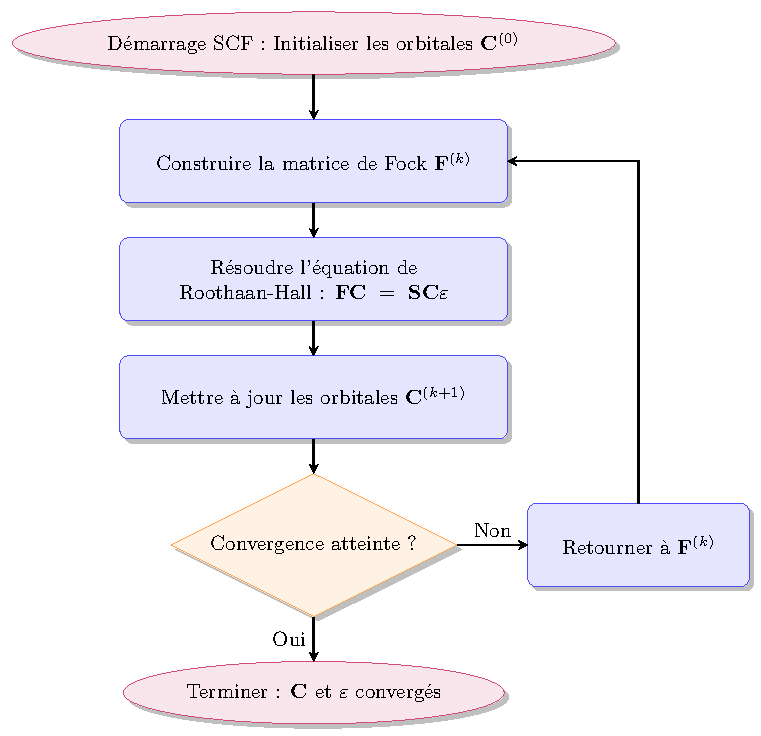
\includegraphics[width=0.6\linewidth]{SCF_Workflow.pdf}
\caption{Workflow détaillé de la procédure SCF (Self-Consistent Field).}
\label{fig:scfworkflow}
\end{figure}

### Accélération - Méthode DIIS

Pour améliorer la convergence, la méthode DIIS (Direct Inversion in the Iterative Subspace) est souvent utilisée. Elle minimise les résidus de chaque itération en combinant les solutions précédentes :
\begin{equation}
e_{m+1} = \sum_{i=1}^m c_i e_i.
\end{equation}
avec des coefficients $c_i$ obtenus en minimisant la norme des résidus.

Lorsque la procédure SCF ne parvient pas à converger, des méthodes d'optimisation directe sont nécessaires. Ces
méthodes sont également nécessaires pour les théories qui pourraient ne pas avoir de solution SCF. Dans de tels cas, des
méthodes telles que la descente de gradient, Newton-Raphson, BFGS ou la méthode de descente géométrique peuvent être utilisées.

On retient que la méthode de Hartree-Fock est la base de nombreuses approches modernes en chimie quantique, servant de point de départ pour des méthodes plus précises qui incorporent la corrélation électronique.

## Corrélation électronique

Malgré l'approximation relativement rudimentaire du champ électronique par la méthode de Hartree-Fock, celle-ci constitue un point de départ solide pour des méthodes plus avancées et capture déjà une grande partie de l’énergie *réelle* du système. La différence entre les valeurs propres réelles de l’Hamiltonien et l’énergie Hartree-Fock est décrite comme l’**énergie de corrélation**.
```{=tex}
\begin{equation}
E_{\text{corrélation}} = E_{\text{exact}} - E_{\text{Hartree-Fock}}.
\end{equation}
```
 D'autres méthodes basées sur la fonction d'état (souvent qualifiées de méthodes **post-Hartree-Fock**) visent à intégrer cette corrélation. Ainsi, la corrélation électronique est essentielle pour améliorer la précision des calculs en chimie quantique.
 
 Les deux types de corrélation sont:

1. **Corrélation statique (forte corrélation)**
   - Présente dans les systèmes où une seule configuration électronique n’est pas suffisante pour décrire correctement l’état quantique.
   - Typique des systèmes avec plusieurs états électroniques dégénérés ou quasi-dégénérés (par exemple, les molécules proches de la dissociation).

2. **Corrélation dynamique (faible corrélation)**
   - Due aux fluctuations instantanées de la répulsion électron-électron.
   - Même lorsque la configuration Hartree-Fock est une bonne approximation qualitative, la corrélation dynamique est nécessaire pour affiner les prédictions quantitatives.

### Méthodes pour inclure la corrélation

1. **Interaction de configuration (CI)**
   - Considère des excitations électroniques au-delà du déterminant de Hartree-Fock.
   - Exemple : CI complète (Full CI), CI singles and doubles (CISD).
```{=tex}
\begin{equation}
|\psi_{\text{CI}}\rangle = C_0 |\psi_0\rangle + \sum_{ia} C_{ia} |\psi_i^a\rangle + \sum_{ijab} C_{ij}^{ab} |\psi_{ij}^{ab}\rangle + \dots .
\end{equation}
```
   - Limitation : Échelle combinatoire (inapplicable aux grands systèmes).

2. **Théorie de la perturbation de Møller-Plesset (MP2)**
   - Approche de la corrélation dynamique en ajoutant un terme perturbatif à l'Hamiltonien de Hartree-Fock.
   - Correction d'ordre 2 donnée par :
```{=tex}
\begin{equation}
E_{\text{MP2}} = \sum_{ijab} \frac{|\langle ab | ij \rangle|^2}{\varepsilon_i + \varepsilon_j - \varepsilon_a - \varepsilon_b} .
\end{equation}
```
   - Avantage : Efficace pour les systèmes faibles à modérément corrélés.
   - Limitation : Ne fonctionne pas bien pour les systèmes fortement corrélés.

3. **Méthodes de Cluster Couplé (CC)**
   - Approche hiérarchique, construisant la fonction d’onde à partir d’un opérateur exponentiel :
\begin{equation}
|\psi_{\text{CC}}\rangle = e^{\hat{T}} |\psi_0\rangle .
\end{equation}

   - $\hat{T}$ est l’opérateur de cluster, décomposé comme suit :
\begin{equation}
\hat{T} = \hat{T}_1 + \hat{T}_2 + \hat{T}_3 + \dots .
\end{equation}

   - Exemple : CCSD (singles et doubles), CCSD(T) (avec correction perturbative des triples).
   - Limitation : Très coûteux pour les grands systèmes.

4. **Méthodes basées sur la DFT (Density Functional Theory) :**
   - Approximations fonctionnelles pour inclure la corrélation électronique.
   - Moins coûteux, mais dépend fortement du choix de la fonctionnelle.

Le \autoref{tab:comparaison} établit une comparaison des méthodes pour inclure la corrélation électronique.

```{=tex}
\begin{table}[h!]
\centering
\caption{Comparaison des méthodes pour inclure la corrélation électronique}
\begin{tabular}{@{}lccc@{}}
\toprule
\textbf{Méthode}       & \textbf{Corrélation incluse} & \textbf{Précision}  & \textbf{Coût computationnel} \\ \midrule
Hartree-Fock           & Aucune                      & Faible              & Faible                       \\
MP2                    & Dynamique uniquement        & Modérée             & $O(N^5)$                     \\
CI (CISD)              & Statique + Dynamique        & Bonne               & $O(N^6)$                     \\
CC (CCSD)              & Statique + Dynamique        & Très bonne          & $O(N^6)$ à $O(N^7)$          \\
DFT                    & Approximative               & Variable            & $O(N^3)$ à $O(N^4)$          \\ \bottomrule
\end{tabular}
\label{tab:comparaison}
\end{table}
```

## Méthodes pour l'état fondamental

Les méthodes pour l'état fondamental visent à résoudre avec précision l'équation de Schrödinger pour les systèmes multi-électroniques, en incluant la corrélation électronique qui manque dans la méthode Hartree-Fock. Ces approches capturent différents niveaux de corrélation, allant de la dynamique à la statique, et offrent un compromis entre précision et coût computationnel.

### Méthodes basées sur la fonction d'état

1. **Interaction de configuration (CI)**
   - Cette méthode construit la fonction d'état comme une combinaison linéaire de déterminants excités :
```{=tex}
\begin{equation}
|\psi_{\text{CI}}\rangle = C_0 |\psi_0\rangle + \sum_{ia} C_{ia} |\psi_i^a\rangle + \sum_{ijab} C_{ij}^{ab} |\psi_{ij}^{ab}\rangle + \dots .
\end{equation}
```
   - **CI complète (Full CI, FCI)**
     - Inclut toutes les excitations possibles.
     - Offre une précision maximale mais a un coût combinatoire ($O(N!)$).
   - **CI tronquée (CI Single, CIS; CI Single and Double, CISD)** 
     - Limite les excitations aux simples (CIS) ou doubles (CISD).
     - CISD est d'ordre $O(N^6)$ mais n'est pas cohérente en taille, ce qui limite son applicabilité pour les grands systèmes.

2. **Théorie de la perturbation de Møller-Plesset (MP2)**
   - Approche basée sur une correction perturbative à la méthode de Hartree-Fock :
```{=tex}
\begin{equation}
E_{\text{MP2}} = \sum_{ijab} \frac{|\langle ab || ij \rangle|^2}{\varepsilon_i + \varepsilon_j - \epsilon_a - \varepsilon_b} .
\end{equation}
```
   - Avantages :
     - Capture efficacement la corrélation dynamique.
     - Échelle modérée ($O(N^5)$).
   - Limites :
     - Inefficace pour les systèmes fortement corrélés.

3. **Cluster Couplé (CC)**
   - Méthode basée sur l'application d'un opérateur exponentiel pour inclure les excitations :
\begin{equation}
|\psi_{\text{CC}}\rangle = e^{\hat{T}} |\psi_0\rangle .
\end{equation}

   - L'opérateur de cluster $\hat{T}$ est défini comme :
\begin{equation}
\hat{T} = \hat{T}_1 + \hat{T}_2 + \hat{T}_3 + \dots .
\end{equation}

   - Variantes :
     - **CCSD** (singles et doubles, $O(N^6)$).
     - **CCSD(T)** (avec triples perturbatifs, $O(N^7)$).
   - Avantages :
     - Très précis pour les systèmes faiblement corrélés.
   - Limites :
     - Coût prohibitif pour les grands systèmes.

Le \autoref{tab:groundstate} présente une comparaison des méthodes d'état fondamental.
```{=tex}
\begin{table}[htpb]
\centering
\caption{Comparaison des méthodes d'état fondamental}
\begin{tabular}{@{}lccc@{}}
\toprule
\textbf{Méthode}       & \textbf{Corrélation incluse} & \textbf{Précision}  & \textbf{Coût computationnel} \\ \midrule
Hartree-Fock           & Aucune                      & Faible              & Faible                       \\
MP2                    & Dynamique uniquement        & Modérée             & $O(N^5)$                     \\
CI (CISD)              & Statique + Dynamique        & Bonne               & $O(N^6)$                     \\
CC (CCSD)              & Statique + Dynamique        & Très bonne          & $O(N^6)$ à $O(N^7)$          \\ \bottomrule
\end{tabular}
\label{tab:groundstate}
\end{table}


\begin{tikzpicture}[
    mybox/.style={draw=black, thick, fill=blue!10, rounded corners, inner sep=10pt},
    title/.style={font=\bfseries}
]

% Box
\node[mybox] (box) {
    \begin{minipage}{0.9\textwidth}
        \textbf{Résumé des méthodes d'état fondamental}
        \begin{itemize}
            \item \textbf{Hartree-Fock :} Point de départ pour les méthodes avancées, mais ne capture pas la corrélation.
            \item \textbf{MP2 :} Approche perturbative efficace pour la corrélation dynamique ($O(N^5)$).
            \item \textbf{CI :} Capture la corrélation statique et dynamique, mais coûteuse ($O(N^6)$).
            \item \textbf{CC :} Méthode hiérarchique précise ($O(N^6)$ à $O(N^7)$).
        \end{itemize}
    \end{minipage}
};

\end{tikzpicture}

```

Les méthodes pour l’état fondamental offrent une hiérarchie de précisions et de coûts computationnels, permettant aux chercheurs de choisir l’approche la plus adaptée selon leurs besoins. 


##  Méthodes pour les états excités

Compte tenu des approximations et des défis liés à la théorie de la structure électronique de l'état fondamental, il n'est pas surprenant que la théorie de la structure électronique des états excités soit plus complexe et nécessite à la fois de nouvelles approches théoriques et davantage de nuances. Alors qu'il n'existe généralement qu'un seul état fondamental global, les états excités sont nombreux, avec des caractéristiques de spin et de symétrie différentes. Ils sont également plus difficiles à optimiser, car ils ne correspondent pas à des minima d'énergie, mais se situent souvent au niveau de points selles (saddle points). 

L'une des approches les plus simples consiste, une fois encore, à examiner les racines supérieures des équations de CI (Interaction de Configuration). Cependant, en fonction de l'ordre des excitations pris en compte dans la CI, cette méthode peut, comme pour l'état fondamental, devenir prohibitivement coûteuse. Trouver un équilibre entre les coûts computationnels, la précision et les aspects physiques spécifiques d'un calcul donné a largement motivé le développement des méthodes pour les états excités. 

Bien qu'il existe des centaines de méthodes possibles pour calculer les propriétés de la chimie quantique des états excités, nous nous concentrerons ici sur les méthodes qui tentent de capturer les effets des relaxations orbitalaires après excitation ainsi que sur certaines des méthodes les plus couramment utilisées pour les états excités. Les relaxations orbitalaires peuvent avoir des conséquences énergétiques significatives, en particulier pour les états de transfert de charge (CT), et elles sont également nécessaires si une méthode peu coûteuse pour les états excités doit jouer un rôle similaire à celui de la théorie Hartree-Fock pour l'état fondamental, en fournissant une base où les effets de corrélation peuvent être ajoutés sur une structure orbitaire déjà relaxée.

### Principales méthodes

1. **Méthode CIS (Configuration Interaction Singles) :**
   - Approche simple qui inclut uniquement des excitations simples depuis l’état fondamental Hartree-Fock.
   - Fonction d’onde approximée :

\begin{equation}
|\psi_{\text{CIS}}\rangle = C_0 |\psi_0\rangle + \sum_{i,a} C_{ia} |\psi_i^a\rangle
\end{equation}

   - Limites :
     - Néglige les corrélations dynamiques.
     - Ne capte pas correctement les transferts de charge.

2. **Théorie de la fonctionnelle de densité dépendant du temps (TDDFT) :**
   - Étend la DFT pour inclure les excitations via une réponse linéaire au potentiel externe.
   - Donne directement les énergies d'excitation :

\begin{equation}
\Delta E = \epsilon_a - \epsilon_i + f_{xc}
\end{equation}

   - $f_{xc}$ : Terme de correction fonctionnelle pour les états excités.
   - Avantages :
     - Efficace en termes de coût computationnel ($O(N^3)$).
     - Bien adaptée pour les excitations localisées.
   - Limites :
     - Moins précise pour les excitations de transfert de charge ou de Rydberg.

3. **Cluster couplé en équation de mouvement (EOM-CCSD) :**
   - Approche hautement précise basée sur le cluster couplé pour l’état fondamental.
   - Fonction d’onde des états excités construite comme une perturbation de l’état fondamental :

\begin{equation}
|\psi_{\text{EOM}}\rangle = R |\psi_{\text{CCSD}}\rangle
\end{equation}

   - Avantages :
     - Capture avec précision les corrélations statiques et dynamiques.
   - Limites :
     - Très coûteux ($O(N^6)$).

4. **Méthodes basées sur des déterminants multiples (MCSCF, CASSCF) :**
   - Approches multiréférentielles adaptées aux systèmes où plusieurs états électroniques participent (corrélation statique forte).
   - Utilisées pour les spectres complexes (métaux de transition, dissociations).


### CIS à orbitales optimisées (OO-CIS)

La méthode **CIS à orbitales optimisées (OO-CIS)** est une extension de la méthode **Configuration Interaction Singles (CIS)**, qui vise à corriger l'une des principales limitations de CIS classique : le manque de relaxation orbitale après excitation. Dans la méthode CIS classique, les orbitales moléculaires utilisées restent celles optimisées pour l'état fondamental Hartree-Fock, ce qui peut entraîner des erreurs significatives, notamment pour les états de transfert de charge (CT) ou les excitations avec de fortes distorsions structurelles.

OO-CIS aborde cette limitation en optimisant simultanément les orbitales moléculaires pour l’état excité ciblé.

#### Fonction d'onde

La fonction d'état OO-CIS est similaire à celle de CIS classique, mais elle est définie dans un espace orbitalaire optimisé :
```{=tex}
\begin{equation}
|\psi_{\text{OO-CIS}}\rangle = C_0 |\psi_0\rangle + \sum_{i,a} C_{ia} |\psi_i^a\rangle ,
\end{equation}
```
où,
- $C_0$ est le coefficient du déterminant de référence (état fondamental Hartree-Fock);
- $C_{ia}$ sont les coefficients associés aux excitations simples d'un électron de l'orbitale occupée $i$ vers l'orbitale inoccupée $a$;
- les orbitales $|\psi_0\rangle$ et $|\psi_i^a\rangle$ sont réoptimisées pour refléter l'état excité.

#### Optimisation des orbitales

L’objectif est de minimiser l'énergie de l'état excité ciblé par rapport aux coefficients $C_{ia}$ et aux orbitales moléculaires. Cela nécessite une approche variationnelle qui résout simultanément :

1. les amplitudes des coefficients de configuration $C_{ia}$,
2. les coefficients des orbitales moléculaires optimisées.

La condition d’orthogonalité entre les orbitales d’occupation et de désexcitation est préservée pendant l’optimisation.

#### Avantages de OO-CIS

1. **Relaxation orbitale incluse**
   - Les orbitales sont optimisées pour mieux représenter l'état excité, ce qui améliore la précision par rapport à CIS classique.

2. **Meilleure description des états de transfert de charge (CT)**
   - Les relaxations orbitalaires permettent de mieux capturer les effets énergétiques associés aux transferts électroniques.

3. **Base pour des méthodes corrélées**
   - OO-CIS peut servir de point de départ pour des méthodes plus sophistiquées, comme EOM-CCSD ou des approches multiréférentielles.

#### Limites

- OO-CIS reste limité aux excitations simples et ne capture pas les corrélations dynamiques.
- L'optimisation conjointe des orbitales et des configurations peut être numériquement coûteuse et nécessite des algorithmes robustes.

En conclusion, OO-CIS est une amélioration significative de CIS, particulièrement utile pour les états excités nécessitant une relaxation orbitale importante. Bien qu'elle ne capture pas tous les effets de corrélation, elle représente une étape intermédiaire efficace entre les méthodes CIS classiques et les approches entièrement corrélées. 

La \autoref{tab:excited_state_methods} établit un comparatif des méthodes pour les états excités.

```{=tex}
\begin{table}[htpb]
\centering
\caption{Comparaison des méthodes pour les états excités}
\begin{tabular}{@{}lccc@{}}
\toprule
\textbf{Méthode}         & \textbf{Type d’excitation}   & \textbf{Précision}   & \textbf{Coût computationnel} \\ \midrule
CIS                      & Simples                     & Faible               & $O(N^3)$                     \\
OO-CIS                   & Simples + Relaxation        & Modérée à Bonne      & $O(N^4)$                     \\
TDDFT                    & Dynamique                   & Modérée              & $O(N^3)$ à $O(N^4)$          \\
EOM-CCSD                 & Statique + Dynamique        & Très bonne           & $O(N^6)$                     \\
MCSCF / CASSCF           & Statique + Dynamique        & Excellente           & Très élevé                    \\ \bottomrule
\end{tabular}
\label{tab:excited_state_methods}
\end{table}


\begin{tikzpicture}[
    mybox/.style={draw=black, thick, fill=yellow!10, rounded corners, inner sep=10pt},
    title/.style={font=\bfseries}
]

% Box
\node[mybox] (box) {
    \begin{minipage}{0.9\textwidth}
        \textbf{Résumé des méthodes pour les états excités :}
        \begin{itemize}
            \item \textbf{CIS :} Simples excitations ($O(N^3)$), mais néglige les corrélations dynamiques.
            \item \textbf{OO-CIS :} Introduit une relaxation orbitale pour mieux décrire les états excités ($O(N^4)$).
            \item \textbf{TDDFT :} Capture efficacement les excitations localisées, mais moins adaptée aux transferts de charge.
            \item \textbf{EOM-CCSD :} Très précis pour les états excités corrélés ($O(N^6)$).
            \item \textbf{MCSCF / CASSCF :} Idéal pour les systèmes fortement corrélés.
        \end{itemize}
    \end{minipage}
};
\end{tikzpicture}

```

Les méthodes pour les états excités varient en termes de précision et de coût computationnel, permettant un choix adapté selon la complexité du système et les objectifs de l'étude. Les approches avancées comme EOM-CCSD offrent une grande précision mais nécessitent des ressources importantes, tandis que TDDFT représente un compromis idéal pour de nombreux systèmes pratiques.

\end{markdown}

\end{document}